\subsubsection{Tangent Bundles}
The tangent bundle of a manifold $\mathcal{M}$ is the union of all the tangent spaces, hence: 
$$T\mathcal{M} = \bigcup\limits_{p\in \mathcal{M}}T_p\mathcal{M}$$
We can define a `natural' (coordinate or chart independent) map $\pi$ from the tangent bundle to the manifold given by $\pi(v) = p, \ \ v \in T_p\mathcal{M}$ (since tangent bundle is the union of tangent spaces, it indeed consists of elements from $\{T_p\SM\}$). The map $\pi$ is sometimes called the \textit{canonical projection}.
Notice that the tangent bundle is just a set, with no structure or anything else. Let us modify this a bit. Suppose we have a chart $(U,\phi)$, then we will have:
$$TU =  \bigcup\limits_{p\in {U}}T_p{U}= \bigcup\limits_{p\in \mathcal{U}}T_p\mathcal{M}$$ 
The last two things can be shown to be equal. Since the set of derivations form a basis for the tangent space at $p$, we can write the tangent vector uniquely as a linear combination:
$$T_p\mathcal{M}\ni v_p = \sum\limits_{i}^n \dot{q}^i(v_p) \pdv{x^i}\Bigg|_p$$
Here, $\dot{q}^i: \pi^{-1}(U)\rightarrow \mathbb{R}$ are $n$ real-valued functions \footnote{The notation is borrowed from Lagrangian formulation of classical mechanics, where the manifold becomes the configuration space of the mechanical system}. Let us also define $q^i:\pi^{-1}(U)\rightarrow \re, {q}^i\equiv x^i\circ \pi = \pi^*x^i$ and $\bar{phi}:\phi^{-1}(U)\rightarrow \re^{2n}$
$$\bar{\phi}(v_p)\equiv \brac{q^1(v_p), q^2(v_p),\ldots,q^n(v_p),\dot{q}^1(v_p), \dot{q}^2(v_p),\ldots,\dot{q}^n(v_p)}$$ 
Note that $\bar{\phi}$ has an inverse such that $\brac{q^1(v_p), q^2(v_p),\ldots,q^n(v_p),\dot{q}^1(v_p), \dot{q}^2(v_p),\ldots,\dot{q}^n(v_p)} \mapsto \sum\limits_{i}^n \dot{q}^i(v_p) \pdv{x^i}\Bigg|_p$ and is thus a bijection. Also, 
\begin{align*}
  q^i(v_p) &= x^i\circ\pi(v_p) = x^i(p)\\
  v_p &= \dot{q}^i(v_p) \pdv{x^i}\Bigg|_p \implies  \dot{q}^i(v_p) = v_p[x^i]
\end{align*}
Thus, the function $\bar{\phi}$ becomes:
$$\bar{\phi}(v_p)\equiv \brac{x^1(p), x^2(p),\ldots,x^n(p),v_p[x^1], v_p[x^2],\ldots,v_p[x^n]}$$ 
\begin{figure}[H]
  \centering 
  

\tikzset{every picture/.style={line width=0.75pt}} %set default line width to 0.75pt        

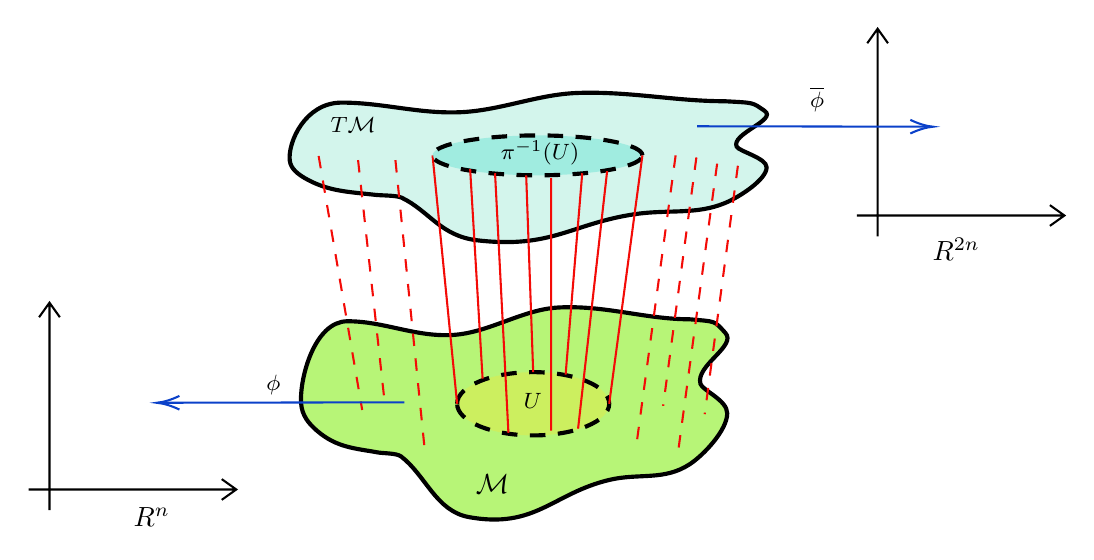
\begin{tikzpicture}[x=0.75pt,y=0.75pt,yscale=-1,xscale=1]
%uncomment if require: \path (0,351); %set diagram left start at 0, and has height of 351

%Shape: Boxed Bezier Curve [id:dp7555542346097139] 
\draw [fill={rgb, 255:red, 211; green, 245; blue, 236 }  ,fill opacity=1 ][line width=1.5]    (391.34,61.94) .. controls (367.37,61.94) and (345.22,57.03) .. (320.2,57.96) .. controls (300.91,58.67) and (282.94,66.54) .. (263.47,67.25) .. controls (243.27,67.98) and (226.53,62.6) .. (206.75,62.6) .. controls (189.05,62.6) and (180.8,81.91) .. (181.76,90.47) .. controls (182.21,94.49) and (185.77,97.27) .. (190.41,99.76) .. controls (201.06,105.48) and (210.83,105.65) .. (223.1,107.06) .. controls (225.93,107.38) and (233.27,107.27) .. (235.59,108.38) .. controls (248.94,114.76) and (254.4,126.91) .. (272.13,128.95) .. controls (308.22,133.11) and (317.45,120.88) .. (348.08,116.35) .. controls (363.96,114) and (377.58,116.74) .. (391.34,111.04) .. controls (398.74,107.97) and (411.53,99.55) .. (411.53,93.79) .. controls (411.53,89.32) and (398.16,86.03) .. (397.11,83.84) .. controls (394.13,77.68) and (416.9,70.96) .. (410.56,66.58) .. controls (404.35,62.3) and (405.76,62.75) .. (391.34,61.94) -- cycle ;
%Shape: Boxed Bezier Curve [id:dp6883735068899058] 
\draw [fill={rgb, 255:red, 158; green, 241; blue, 71 }  ,fill opacity=0.74 ][line width=1.5]    (374.5,167) .. controls (353.09,167) and (333.29,160.03) .. (310.94,161.34) .. controls (293.71,162.35) and (277.65,173.54) .. (260.26,174.55) .. controls (242.2,175.59) and (227.24,167.94) .. (209.57,167.94) .. controls (193.76,167.94) and (186.39,195.39) .. (187.24,207.57) .. controls (187.64,213.29) and (190.83,217.23) .. (194.97,220.77) .. controls (204.49,228.9) and (213.22,229.14) .. (224.18,231.15) .. controls (226.71,231.61) and (233.27,231.46) .. (235.34,233.04) .. controls (247.26,242.1) and (252.15,259.38) .. (267.99,262.28) .. controls (300.24,268.18) and (308.48,250.8) .. (335.85,244.36) .. controls (350.04,241.02) and (362.21,244.91) .. (374.5,236.81) .. controls (381.12,232.45) and (392.54,220.47) .. (392.54,212.28) .. controls (392.54,205.93) and (380.6,201.25) .. (379.66,198.13) .. controls (377,189.38) and (397.34,179.82) .. (391.68,173.6) .. controls (386.13,167.51) and (387.39,168.15) .. (374.5,167) -- cycle ;
%Shape: Ellipse [id:dp7913055919056734] 
\draw  [fill={rgb, 255:red, 245; green, 230; blue, 53 }  ,fill opacity=0.35 ][dash pattern={on 5.63pt off 4.5pt}][line width=1.5]  (262.41,207.7) .. controls (262.41,199.28) and (278.81,192.46) .. (299.05,192.46) .. controls (319.28,192.46) and (335.68,199.28) .. (335.68,207.7) .. controls (335.68,216.12) and (319.28,222.95) .. (299.05,222.95) .. controls (278.81,222.95) and (262.41,216.12) .. (262.41,207.7) -- cycle ;
%Straight Lines [id:da38840826454836663] 
\draw [color={rgb, 255:red, 243; green, 11; blue, 7 }  ,draw opacity=1 ][line width=0.75]    (250.56,88.02) -- (262.41,207.7) ;
%Shape: Ellipse [id:dp3372595327826894] 
\draw  [fill={rgb, 255:red, 119; green, 230; blue, 215 }  ,fill opacity=0.55 ][dash pattern={on 5.63pt off 4.5pt}][line width=1.5]  (351.68,88.02) .. controls (351.68,82.72) and (329.05,78.41) .. (301.12,78.41) .. controls (273.2,78.41) and (250.56,82.72) .. (250.56,88.02) .. controls (250.56,93.33) and (273.2,97.63) .. (301.12,97.63) .. controls (329.05,97.63) and (351.68,93.33) .. (351.68,88.02) -- cycle ;
%Straight Lines [id:da561591323588785] 
\draw [color={rgb, 255:red, 243; green, 11; blue, 7 }  ,draw opacity=1 ][line width=0.75]    (351.68,88.02) -- (335.68,207.7) ;
%Straight Lines [id:da690868976884767] 
\draw [color={rgb, 255:red, 243; green, 11; blue, 7 }  ,draw opacity=1 ][line width=0.75]    (334.68,95.63) -- (320.68,219.7) ;
%Straight Lines [id:da0643786859358153] 
\draw [color={rgb, 255:red, 243; green, 11; blue, 7 }  ,draw opacity=1 ][line width=0.75]    (280.68,96.63) -- (287.12,221.7) ;
%Straight Lines [id:da5276401921204039] 
\draw [color={rgb, 255:red, 243; green, 11; blue, 7 }  ,draw opacity=1 ][line width=0.75]    (307.72,98.81) -- (307.68,220.63) ;
%Straight Lines [id:da02591874235055658] 
\draw [color={rgb, 255:red, 243; green, 11; blue, 7 }  ,draw opacity=1 ][line width=0.75]    (268.68,94.63) -- (274.68,195.63) ;
%Straight Lines [id:da13234226839924923] 
\draw [color={rgb, 255:red, 243; green, 11; blue, 7 }  ,draw opacity=1 ][line width=0.75]    (295.68,97.63) -- (299.05,192.46) ;
%Straight Lines [id:da10881113373921192] 
\draw [color={rgb, 255:red, 243; green, 11; blue, 7 }  ,draw opacity=1 ][line width=0.75]    (322.68,96.63) -- (314.68,193.63) ;
%Straight Lines [id:da1622212363017358] 
\draw [color={rgb, 255:red, 243; green, 11; blue, 7 }  ,draw opacity=1 ][line width=0.75]  [dash pattern={on 4.5pt off 4.5pt}]  (367.68,88.02) -- (348.68,228.3) ;
%Straight Lines [id:da48330270456949853] 
\draw [color={rgb, 255:red, 243; green, 11; blue, 7 }  ,draw opacity=1 ][line width=0.75]  [dash pattern={on 4.5pt off 4.5pt}]  (377.68,89.02) -- (361.68,208.7) ;
%Straight Lines [id:da2990883543810654] 
\draw [color={rgb, 255:red, 243; green, 11; blue, 7 }  ,draw opacity=1 ][line width=0.75]  [dash pattern={on 4.5pt off 4.5pt}]  (195.68,88.3) -- (216.68,210.7) ;
%Straight Lines [id:da95060641908313] 
\draw [color={rgb, 255:red, 243; green, 11; blue, 7 }  ,draw opacity=1 ][line width=0.75]  [dash pattern={on 4.5pt off 4.5pt}]  (214.68,90.3) -- (227.68,208.7) ;
%Straight Lines [id:da7748858791112593] 
\draw [color={rgb, 255:red, 243; green, 11; blue, 7 }  ,draw opacity=1 ][line width=0.75]  [dash pattern={on 4.5pt off 4.5pt}]  (232.68,90.3) -- (246.68,228.7) ;
%Straight Lines [id:da23543355149656475] 
\draw [color={rgb, 255:red, 243; green, 11; blue, 7 }  ,draw opacity=1 ][line width=0.75]  [dash pattern={on 4.5pt off 4.5pt}]  (387.68,92.02) -- (368.68,232.3) ;
%Straight Lines [id:da252934263423064] 
\draw [color={rgb, 255:red, 243; green, 11; blue, 7 }  ,draw opacity=1 ][line width=0.75]  [dash pattern={on 4.5pt off 4.5pt}]  (397.68,93.02) -- (381.68,212.7) ;
%Shape: Axis 2D [id:dp028583688594270185] 
\draw  (56,249) -- (156,249)(66,159) -- (66,259) (149,244) -- (156,249) -- (149,254) (61,166) -- (66,159) -- (71,166)  ;
%Shape: Axis 2D [id:dp8970413200540654] 
\draw  (455,117) -- (555,117)(465,27) -- (465,127) (548,112) -- (555,117) -- (548,122) (460,34) -- (465,27) -- (470,34)  ;
%Straight Lines [id:da828009539651172] 
\draw [color={rgb, 255:red, 11; green, 65; blue, 201 }  ,draw opacity=1 ]   (237,207) -- (119.68,207.21) ;
\draw [shift={(117.68,207.22)}, rotate = 359.9] [color={rgb, 255:red, 11; green, 65; blue, 201 }  ,draw opacity=1 ][line width=0.75]    (10.93,-3.29) .. controls (6.95,-1.4) and (3.31,-0.3) .. (0,0) .. controls (3.31,0.3) and (6.95,1.4) .. (10.93,3.29)   ;
%Straight Lines [id:da45797751736499215] 
\draw [color={rgb, 255:red, 11; green, 65; blue, 201 }  ,draw opacity=1 ]   (378,74) -- (489.68,74.21) ;
\draw [shift={(491.68,74.22)}, rotate = 180.11] [color={rgb, 255:red, 11; green, 65; blue, 201 }  ,draw opacity=1 ][line width=0.75]    (10.93,-3.29) .. controls (6.95,-1.4) and (3.31,-0.3) .. (0,0) .. controls (3.31,0.3) and (6.95,1.4) .. (10.93,3.29)   ;

% Text Node
\draw (270,240.4) node [anchor=north west][inner sep=0.75pt]    {$\mathcal{M}$};
% Text Node
\draw (282,79.4) node [anchor=north west][inner sep=0.75pt]  [font=\footnotesize]  {$\pi ^{-1}( U)$};
% Text Node
\draw (293,201.4) node [anchor=north west][inner sep=0.75pt]  [font=\footnotesize]  {$U$};
% Text Node
\draw (200,68.4) node [anchor=north west][inner sep=0.75pt]  [font=\footnotesize]  {$T\mathcal{M}$};
% Text Node
\draw (105,256.4) node [anchor=north west][inner sep=0.75pt]    {$\mathbb{R}^{n}$};
% Text Node
\draw (490,126.4) node [anchor=north west][inner sep=0.75pt]    {$\mathbb{R}^{2n}$};
% Text Node
\draw (169,192.4) node [anchor=north west][inner sep=0.75pt]  [font=\footnotesize]  {$\phi $};
% Text Node
\draw (431,53.4) node [anchor=north west][inner sep=0.75pt]  [font=\footnotesize]  {$\overline{\phi }$};


\end{tikzpicture}

  \caption{Diagram showing the chart $\brac{\pi^{-1}(U),\bar{\phi}}$. The red lines represent the tangent space at each point of the manifold. Solid lines represent the tangent spaces for points belonging in $U$}
\end{figure}
\begin{lemma}
  The pair $\brac{\pi^{-1}(U),\bar{\phi}}$ is a chart on $T\SM$, often called the \textit{bundle chart}.
\end{lemma}
% \textit{Proof.} To prove that it is indeed a chart, we need to check if there exists a homeomorphism between the open sets $\pi^{-1}(U)$ and $\bar{\phi}(\pi^{-1}(U))$.\\[0.2cm] Firstly, note that $\bar{\phi}(\pi^{-1}(U)) = \phi(U)\times \re^n$. To understand this, observe that $\bar{\phi}$ acts on a tangent vector $v_p$, giving a $2n$ component vector, whose first $n$ components $\{q^i(v_p)\}$ are simply the coordinates of point $p$ (since $\pi$ takes $v_p$ to $p$) and hence these belong to $\phi(U)$. The last $n$ components can be arbitrary real numbers and hence belong to $\re^n$. Now, since $\re^n$ and $\phi(U)$ both are open sets, $\phi(U)\times \re^n$ is also open.  \\[0.2cm]
% Now, let us check if $\bar{\phi}$ is a homeomorphism. The components of $\bar{\phi}$ are smooth maps and hence $\bar{\phi}$ is smooth, hence continuous. \textcolor{red}{PROOF LEFT!}
The tangent bundle can also be shown to be \textit{Hausdorff} and \textit{second countable}. Well, tangent bundles are a special case of something called a fibre bundle. 
\begin{figure}[H]
  \centering 
  

\tikzset{every picture/.style={line width=0.75pt}} %set default line width to 0.75pt        

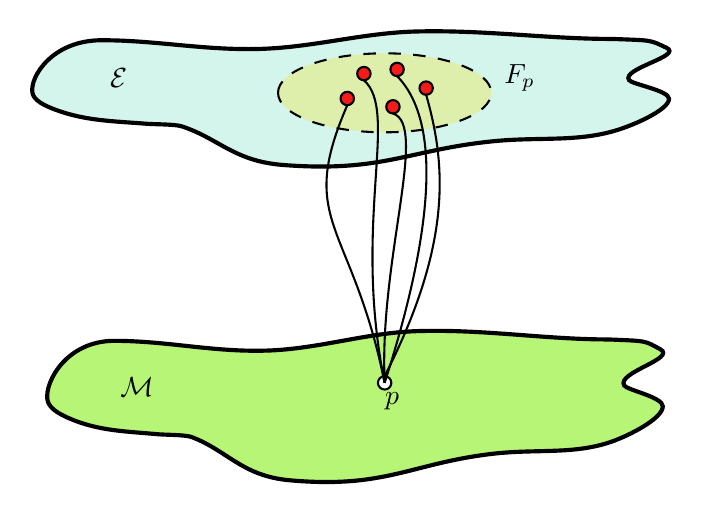
\begin{tikzpicture}[x=0.75pt,y=0.75pt,yscale=-1,xscale=1]
%uncomment if require: \path (0,351); %set diagram left start at 0, and has height of 351

%Shape: Boxed Bezier Curve [id:dp1046279221987515] 
\draw [fill={rgb, 255:red, 211; green, 245; blue, 236 }  ,fill opacity=1 ][line width=1.5]    (437.84,58.55) .. controls (405.85,58.55) and (376.27,54.11) .. (342.87,54.95) .. controls (317.13,55.59) and (293.14,62.72) .. (267.15,63.36) .. controls (240.17,64.03) and (217.83,59.16) .. (191.43,59.16) .. controls (167.8,59.16) and (156.79,76.64) .. (158.06,84.39) .. controls (158.66,88.04) and (163.42,90.55) .. (169.61,92.81) .. controls (183.83,97.99) and (196.88,98.14) .. (213.25,99.42) .. controls (217.04,99.71) and (226.83,99.61) .. (229.93,100.62) .. controls (247.74,106.39) and (255.04,117.4) .. (278.7,119.25) .. controls (326.89,123.01) and (339.2,111.93) .. (380.09,107.83) .. controls (401.29,105.7) and (419.47,108.19) .. (437.84,103.02) .. controls (447.73,100.25) and (464.79,92.62) .. (464.79,87.4) .. controls (464.79,83.35) and (446.95,80.37) .. (445.54,78.39) .. controls (441.57,72.81) and (471.96,66.72) .. (463.51,62.76) .. controls (455.21,58.88) and (457.09,59.29) .. (437.84,58.55) -- cycle ;
%Shape: Ellipse [id:dp7051113917362648] 
\draw  [fill={rgb, 255:red, 245; green, 230; blue, 53 }  ,fill opacity=0.35 ][dash pattern={on 4.5pt off 4.5pt}] (276.41,84.49) .. controls (276.41,73.98) and (299.41,65.46) .. (327.78,65.46) .. controls (356.14,65.46) and (379.14,73.98) .. (379.14,84.49) .. controls (379.14,95) and (356.14,103.52) .. (327.78,103.52) .. controls (299.41,103.52) and (276.41,95) .. (276.41,84.49) -- cycle ;
%Shape: Boxed Bezier Curve [id:dp6248237388540854] 
\draw [fill={rgb, 255:red, 158; green, 241; blue, 71 }  ,fill opacity=0.74 ][line width=1.5]    (435.74,203.32) .. controls (404.82,203.32) and (376.22,198.36) .. (343.93,199.29) .. controls (319.05,200.01) and (295.86,207.98) .. (270.73,208.7) .. controls (244.65,209.44) and (223.04,203.99) .. (197.53,203.99) .. controls (174.68,203.99) and (164.04,223.54) .. (165.27,232.2) .. controls (165.85,236.28) and (170.45,239.09) .. (176.44,241.61) .. controls (190.18,247.39) and (202.79,247.57) .. (218.62,249) .. controls (222.28,249.33) and (231.75,249.21) .. (234.75,250.34) .. controls (251.96,256.79) and (259.02,269.1) .. (281.89,271.16) .. controls (328.48,275.36) and (340.38,262.98) .. (379.91,258.4) .. controls (400.41,256.02) and (417.98,258.79) .. (435.74,253.03) .. controls (445.3,249.92) and (461.8,241.4) .. (461.8,235.56) .. controls (461.8,231.04) and (444.55,227.71) .. (443.19,225.49) .. controls (439.35,219.26) and (468.73,212.45) .. (460.56,208.02) .. controls (452.54,203.68) and (454.35,204.14) .. (435.74,203.32) -- cycle ;
%Shape: Circle [id:dp6027797339068129] 
\draw  [fill={rgb, 255:red, 255; green, 255; blue, 255 }  ,fill opacity=1 ] (324.55,224.22) .. controls (324.55,222.44) and (325.99,221) .. (327.78,221) .. controls (329.56,221) and (331,222.44) .. (331,224.22) .. controls (331,226.01) and (329.56,227.45) .. (327.78,227.45) .. controls (325.99,227.45) and (324.55,226.01) .. (324.55,224.22) -- cycle ;
%Shape: Circle [id:dp7978124382575595] 
\draw  [fill={rgb, 255:red, 245; green, 27; blue, 27 }  ,fill opacity=1 ] (314.55,75.22) .. controls (314.55,73.44) and (315.99,72) .. (317.78,72) .. controls (319.56,72) and (321,73.44) .. (321,75.22) .. controls (321,77.01) and (319.56,78.45) .. (317.78,78.45) .. controls (315.99,78.45) and (314.55,77.01) .. (314.55,75.22) -- cycle ;
%Shape: Circle [id:dp2405724773178366] 
\draw  [fill={rgb, 255:red, 245; green, 27; blue, 27 }  ,fill opacity=1 ] (328.55,91.22) .. controls (328.55,89.44) and (329.99,88) .. (331.78,88) .. controls (333.56,88) and (335,89.44) .. (335,91.22) .. controls (335,93.01) and (333.56,94.45) .. (331.78,94.45) .. controls (329.99,94.45) and (328.55,93.01) .. (328.55,91.22) -- cycle ;
%Shape: Circle [id:dp15559748198633383] 
\draw  [fill={rgb, 255:red, 245; green, 27; blue, 27 }  ,fill opacity=1 ] (330.55,73.22) .. controls (330.55,71.44) and (331.99,70) .. (333.78,70) .. controls (335.56,70) and (337,71.44) .. (337,73.22) .. controls (337,75.01) and (335.56,76.45) .. (333.78,76.45) .. controls (331.99,76.45) and (330.55,75.01) .. (330.55,73.22) -- cycle ;
%Shape: Circle [id:dp9974828834451859] 
\draw  [fill={rgb, 255:red, 245; green, 27; blue, 27 }  ,fill opacity=1 ] (344.55,82.22) .. controls (344.55,80.44) and (345.99,79) .. (347.78,79) .. controls (349.56,79) and (351,80.44) .. (351,82.22) .. controls (351,84.01) and (349.56,85.45) .. (347.78,85.45) .. controls (345.99,85.45) and (344.55,84.01) .. (344.55,82.22) -- cycle ;
%Shape: Circle [id:dp7618982493592206] 
\draw  [fill={rgb, 255:red, 245; green, 27; blue, 27 }  ,fill opacity=1 ] (306.55,87.22) .. controls (306.55,85.44) and (307.99,84) .. (309.78,84) .. controls (311.56,84) and (313,85.44) .. (313,87.22) .. controls (313,89.01) and (311.56,90.45) .. (309.78,90.45) .. controls (307.99,90.45) and (306.55,89.01) .. (306.55,87.22) -- cycle ;
%Curve Lines [id:da05883862390293093] 
\draw    (309.78,90.45) .. controls (285,147.53) and (312,146.53) .. (327.78,224.22) ;
%Curve Lines [id:da18762006209771054] 
\draw    (317.78,78.45) .. controls (335,93.53) and (312,146.53) .. (327.78,224.22) ;
%Curve Lines [id:da37581019078658384] 
\draw    (333.78,76.45) .. controls (355,98.18) and (351.78,149.18) .. (327.78,224.22) ;
%Curve Lines [id:da19009776774897946] 
\draw    (347.78,85.45) .. controls (357,117.9) and (361,155.9) .. (327.78,221) ;
%Curve Lines [id:da2576706771011591] 
\draw    (331.78,94.45) .. controls (349,99.9) and (325,164.9) .. (327.78,224.22) ;

% Text Node
\draw (194,71.4) node [anchor=north west][inner sep=0.75pt]    {$\mathcal{E}$};
% Text Node
\draw (199,220.4) node [anchor=north west][inner sep=0.75pt]    {$\mathcal{M}$};
% Text Node
\draw (326.55,227.62) node [anchor=north west][inner sep=0.75pt]    {$p$};
% Text Node
\draw (384,69.4) node [anchor=north west][inner sep=0.75pt]    {$F_{p}$};


\end{tikzpicture}

  \caption{Diagram showing the base space, total space and the fibre of a point $p$}
\end{figure}
\begin{definition}[Bundle]
  Given a map $\pi: \mathcal{E}\rightarrow M$, the inverse image $pi^{-1}(p)$ to be the \textit{fibre} at $p\in \mathcal{M}$, denoted as $E_p$. For two maps $\pi: \mathcal{E}\rightarrow M$ and $\pi: \mathcal{E}'\rightarrow M$, a map $\phi$ is said to be fibre-preserving if $\phi(E_p)\subset E_p'$.\\[0.2cm]
  A bundle is a triple $(\mathcal{E},\mathcal{M},\pi)$ consisting of manifolds $\mathcal{M}$ which is called the \textit{base space} and the manifold $\mathcal{E}$, called the \textit{total space} and $\pi$ is a continuous, surjective map from the total space to the base space.  
\end{definition}

\begin{figure}[H]
  \centering 
  

% Pattern Info
 
\tikzset{
pattern size/.store in=\mcSize, 
pattern size = 5pt,
pattern thickness/.store in=\mcThickness, 
pattern thickness = 0.3pt,
pattern radius/.store in=\mcRadius, 
pattern radius = 1pt}
\makeatletter
\pgfutil@ifundefined{pgf@pattern@name@_n2wu1tgz5}{
\pgfdeclarepatternformonly[\mcThickness,\mcSize]{_n2wu1tgz5}
{\pgfqpoint{0pt}{0pt}}
{\pgfpoint{\mcSize+\mcThickness}{\mcSize+\mcThickness}}
{\pgfpoint{\mcSize}{\mcSize}}
{
\pgfsetcolor{\tikz@pattern@color}
\pgfsetlinewidth{\mcThickness}
\pgfpathmoveto{\pgfqpoint{0pt}{0pt}}
\pgfpathlineto{\pgfpoint{\mcSize+\mcThickness}{\mcSize+\mcThickness}}
\pgfusepath{stroke}
}}
\makeatother
\tikzset{every picture/.style={line width=0.75pt}} %set default line width to 0.75pt        

\begin{tikzpicture}[x=0.75pt,y=0.75pt,yscale=-1,xscale=1]
%uncomment if require: \path (0,351); %set diagram left start at 0, and has height of 351

%Shape: Boxed Bezier Curve [id:dp12157575364814821] 
\draw [fill={rgb, 255:red, 171; green, 85; blue, 240 }  ,fill opacity=0.37 ][line width=1.5]    (370.11,211.58) .. controls (350.57,211.58) and (332.5,205.11) .. (312.1,206.33) .. controls (296.38,207.27) and (281.73,217.64) .. (265.86,218.57) .. controls (249.38,219.54) and (235.73,212.45) .. (219.61,212.45) .. controls (205.18,212.45) and (198.46,237.89) .. (199.23,249.18) .. controls (199.6,254.48) and (202.51,258.14) .. (206.29,261.42) .. controls (214.97,268.96) and (222.94,269.18) .. (232.94,271.04) .. controls (235.25,271.47) and (241.23,271.33) .. (243.13,272.79) .. controls (254,281.19) and (258.46,297.21) .. (272.91,299.9) .. controls (302.34,305.37) and (309.86,289.25) .. (334.84,283.29) .. controls (347.79,280.19) and (358.89,283.8) .. (370.11,276.29) .. controls (376.15,272.25) and (386.57,261.15) .. (386.57,253.55) .. controls (386.57,247.67) and (375.67,243.32) .. (374.81,240.43) .. controls (372.39,232.32) and (390.95,223.46) .. (385.78,217.7) .. controls (380.72,212.05) and (381.87,212.64) .. (370.11,211.58) -- cycle ;
%Shape: Boxed Bezier Curve [id:dp5903223694774149] 
\draw [fill={rgb, 255:red, 211; green, 245; blue, 236 }  ,fill opacity=1 ][line width=1.5]    (257.23,51.98) .. controls (240.51,51.98) and (225.05,45.83) .. (207.6,46.99) .. controls (194.14,47.88) and (181.61,57.75) .. (168.02,58.64) .. controls (153.93,59.56) and (142.25,52.81) .. (128.45,52.81) .. controls (116.1,52.81) and (110.35,77.02) .. (111.01,87.76) .. controls (111.33,92.81) and (113.82,96.29) .. (117.05,99.41) .. controls (124.48,106.58) and (131.3,106.79) .. (139.86,108.56) .. controls (141.83,108.97) and (146.95,108.83) .. (148.57,110.23) .. controls (157.88,118.22) and (161.7,133.46) .. (174.06,136.02) .. controls (199.24,141.23) and (205.68,125.89) .. (227.05,120.21) .. controls (238.13,117.27) and (247.63,120.7) .. (257.23,113.56) .. controls (262.4,109.71) and (271.31,99.15) .. (271.31,91.92) .. controls (271.31,86.32) and (261.99,82.19) .. (261.25,79.44) .. controls (259.18,71.72) and (275.06,63.29) .. (270.64,57.81) .. controls (266.31,52.43) and (267.29,52.99) .. (257.23,51.98) -- cycle ;
%Shape: Ellipse [id:dp9273591952560972] 
\draw  [fill={rgb, 255:red, 248; green, 231; blue, 28 }  ,fill opacity=0.55 ][dash pattern={on 4.5pt off 4.5pt}] (178.91,91.74) .. controls (178.91,77.94) and (190.42,66.76) .. (204.62,66.76) .. controls (218.81,66.76) and (230.32,77.94) .. (230.32,91.74) .. controls (230.32,105.54) and (218.81,116.72) .. (204.62,116.72) .. controls (190.42,116.72) and (178.91,105.54) .. (178.91,91.74) -- cycle ;
%Straight Lines [id:da5917108377220306] 
\draw    (204.62,91.74) -- (289.43,231.97) ;
\draw [shift={(290.47,233.68)}, rotate = 238.83] [color={rgb, 255:red, 0; green, 0; blue, 0 }  ][line width=0.75]    (10.93,-3.29) .. controls (6.95,-1.4) and (3.31,-0.3) .. (0,0) .. controls (3.31,0.3) and (6.95,1.4) .. (10.93,3.29)   ;
%Shape: Boxed Bezier Curve [id:dp8187304109064342] 
\draw [fill={rgb, 255:red, 126; green, 211; blue, 33 }  ,fill opacity=0.55 ][line width=1.5]    (342.68,47.24) .. controls (359.39,47.24) and (374.85,41.09) .. (392.31,42.25) .. controls (405.76,43.14) and (418.3,53.01) .. (431.88,53.9) .. controls (445.98,54.82) and (457.66,48.07) .. (471.45,48.07) .. controls (483.8,48.07) and (489.55,72.28) .. (488.89,83.02) .. controls (488.58,88.06) and (486.09,91.55) .. (482.85,94.67) .. controls (475.42,101.84) and (468.6,102.05) .. (460.05,103.82) .. controls (458.07,104.23) and (452.95,104.09) .. (451.33,105.48) .. controls (442.02,113.48) and (438.21,128.72) .. (425.84,131.28) .. controls (400.66,136.49) and (394.22,121.15) .. (372.86,115.47) .. controls (361.77,112.52) and (352.28,115.96) .. (342.68,108.81) .. controls (337.51,104.97) and (328.59,94.41) .. (328.59,87.18) .. controls (328.59,81.58) and (337.91,77.45) .. (338.65,74.7) .. controls (340.72,66.98) and (324.84,58.55) .. (329.26,53.06) .. controls (333.6,47.69) and (332.62,48.25) .. (342.68,47.24) -- cycle ;
%Shape: Ellipse [id:dp8365647196815513] 
\draw  [fill={rgb, 255:red, 119; green, 230; blue, 215 }  ,fill opacity=0.55 ][dash pattern={on 4.5pt off 4.5pt}] (419.78,86.15) .. controls (419.78,70.83) and (406.97,58.41) .. (391.17,58.41) .. controls (375.37,58.41) and (362.56,70.83) .. (362.56,86.15) .. controls (362.56,101.46) and (375.37,113.88) .. (391.17,113.88) .. controls (406.97,113.88) and (419.78,101.46) .. (419.78,86.15) -- cycle ;
%Straight Lines [id:da35241639641855826] 
\draw    (391.17,86.15) -- (293.93,233.16) ;
\draw [shift={(292.83,234.83)}, rotate = 303.48] [color={rgb, 255:red, 0; green, 0; blue, 0 }  ][line width=0.75]    (10.93,-3.29) .. controls (6.95,-1.4) and (3.31,-0.3) .. (0,0) .. controls (3.31,0.3) and (6.95,1.4) .. (10.93,3.29)   ;
%Shape: Path Data [id:dp7406886474424567] 
\draw  [pattern=_n2wu1tgz5,pattern size=6pt,pattern thickness=0.75pt,pattern radius=0pt, pattern color={rgb, 255:red, 0; green, 0; blue, 0}][dash pattern={on 4.5pt off 4.5pt}] (386.43,94.03) .. controls (391.01,99.84) and (392.48,107) .. (391.17,113.88) .. controls (382.28,113.36) and (373.91,109.49) .. (368.41,102.52) .. controls (364.09,97.04) and (362.22,90.5) .. (362.59,83.97) .. controls (371.79,83.43) and (380.8,86.9) .. (386.43,94.03) -- cycle ;
%Straight Lines [id:da9966230012431939] 
\draw    (204.62,91.74) -- (376.68,92.88) ;
\draw [shift={(378.68,92.89)}, rotate = 180.38] [color={rgb, 255:red, 0; green, 0; blue, 0 }  ][line width=0.75]    (10.93,-3.29) .. controls (6.95,-1.4) and (3.31,-0.3) .. (0,0) .. controls (3.31,0.3) and (6.95,1.4) .. (10.93,3.29)   ;

% Text Node
\draw (292.49,236.51) node [anchor=north west][inner sep=0.75pt]    {$p$};
% Text Node
\draw (226.87,156.29) node [anchor=north west][inner sep=0.75pt]    {$\pi $};
% Text Node
\draw (95.02,18.65) node [anchor=north west][inner sep=0.75pt]  [font=\Large]  {$\mathcal{E}$};
% Text Node
\draw (488.97,21.5) node [anchor=north west][inner sep=0.75pt]  [font=\Large]  {$\mathcal{E} '$};
% Text Node
\draw (393.75,239.63) node [anchor=north west][inner sep=0.75pt]  [font=\Large]  {$\mathcal{M}$};
% Text Node
\draw (139.69,63.53) node [anchor=north west][inner sep=0.75pt]  [font=\scriptsize]  {$\pi ^{-1}(\{p\})$};
% Text Node
\draw (414.35,60.69) node [anchor=north west][inner sep=0.75pt]  [font=\scriptsize]  {$\pi ^{\prime -1}(\{p\})$};
% Text Node
\draw (343.15,159.14) node [anchor=north west][inner sep=0.75pt]    {$\pi '$};
% Text Node
\draw (296.03,73.78) node [anchor=north west][inner sep=0.75pt]    {$\phi $};


\end{tikzpicture}

  \caption{Commutative diagram for a bundle, showing the fibre preserving map $\phi$}
\end{figure}
\noindent
Fibres can be thought of as points in $\mathcal{E}$ which `strings' together with $p$ in $\mathcal{M}$ (hence the name bundle, like a bundle of strings perhaps...) In a bundle, different points of the base manifold may have (topologically) different fibres. If all points have a fibre, which is togologically equivalent to a single space, say $F$, then we call that bundle a \textit{fibre bundle}. In other words, fibre bundles have a single fibre. \\[0.3cm]
We now define a section of a bundle. Given a bundle $(\mathcal{E}, \mathcal{M}, \pi)$, the section is a map $\sigma: \mathcal{M}\rightarrow \mathcal{E}$ such that $\pi \circ \sigma = \mathds{1}_\mathcal{M}$, the identity map of the base space. What it means that, this map $\sigma$ takes $p$ to some point in the fibre $F_p$ such that when $\pi$ is acted on $\sigma(p)$, we obtain the same point $p$.\\[0.2cm]
Okay, so what was this thing really needed for? Well, we had earlier seen the tangent bundle, which we had written as $T\mathcal{M}$. More appropriately, we should have written it as $(T\mathcal{M}, \mathcal{M}, \pi)$. Then a vector field is nothing but a section of the tangent bundle which assigns a tangent vector (belonging to the tangent space) to each point $p$ in the manifold.